\documentclass[a4paper]{report}   

\usepackage[utf8]{inputenc}
\usepackage[francais]{babel}

\usepackage{multirow}

\usepackage{graphicx}
\usepackage{hyperref}

\usepackage{enumerate}

\title{Détection d'anomalies de classification dans l'IoT via Machine Learning}
\author{Antoine Urban, Yohan Chalier}
\date{\today}

\renewcommand{\arraystretch}{1.2}

\begin{document}

\begin{titlepage}
	\centering
	\vspace{1cm}
	{\scshape\LARGE Télécom ParisTech \par}
	\vspace{1cm}
	{\scshape\Large Projet de filière SR2I \par}
	\vspace{1.5cm}
	{\huge\bfseries Détection d'anomalies de classification dans l'IoT via Machine Learning\par}
	\vspace{2cm}
	{\Large\itshape Antoine Urban, Yohan Chalier \par}
	\vfill
	encadré par\par
	Jean-Philippe \textsc{Monteuuis}\par
	Houda \textsc{Labiod}
	\vfill

% Bottom of the page
	{\large \today\par}
\end{titlepage}



\begin{abstract}
\end{abstract}

\chapter{Démarche et stratégie}

\section{Première implémentation}

\subsection{Objectif}

En premier lieu, nous souhaitions commencer par une vision globale des données et du travail à effectuer. Nous disposions d'une base de données contenant des mesures de voiture, provenant de \href{http://www.carqueryapi.com}{CarQuery}, et contenant 54808 lignes complètes. Dans cette partie, nous allons nous efforcer d'obtenir une première fonction de classification se basant sur des critères très simple : des régions de décision rectangulaires et arbitraires.

\subsection{Mise en {\oe}uvre}

Puisque l'objectif de cette étude est la détection d'anomalies dans la mesure de longueur et de largeur, nous avons extrait les deux colonnes correspondantes dans une DataFrame du module \href{http://pandas.pydata.org}{Pandas}, en Python.

Après un premier affichage des données, il est apparu que beaucoup de points apparaissaient en plusieurs fois, aussi la séparation de la base de données en points uniques et points non-uniques se révéla pertinente. Cela permit de réduire le nombre de lignes à 5026.

Manuellement, nous avons alors défini des zones simples (rectangulaires) en tant que régions de décision (Table \ref{regions_decision_manuelles_valeurs}). Ces zones ont été définies au jugé, afin d'encadrer le plus de points valides sans toutefois englober une zone de l'espace trop large.

\begin{table}[h]
\centering
\begin{tabular}{llll}
cadre & validité & intervalle de longueur & intervalle de largeur \\
\hline
vert & non-malicieux & 3 à 6,5 mètres & 1,4 à 2,4 mètres \\
gris & malicieux & 3 à 4,1 mètres & 2,05 à 2,4 mètres \\
gris & malicieux & 5,25 à 6,5 mètres & 1,4 à 1,65 mètres \\
\end{tabular}
\caption{Dimensions des régions de décision arbitraires\label{regions_decision_manuelles_valeurs}}
\end{table}

%TODO Parler des records de taille

Hors de la zone verte, et dans les deux cadres gris, nous avons alors généré aléatoirement 700 points définis comme malicieux. La Figure \ref{regions_decision_manuelles_plot} représente l'affichage de tous les points décrits plus tôt ainsi que des régions de décision. Ainsi faite, notre classification possède, sur le jeu d'entraînement, une précision de 97,57\%.

\begin{figure}
\centering
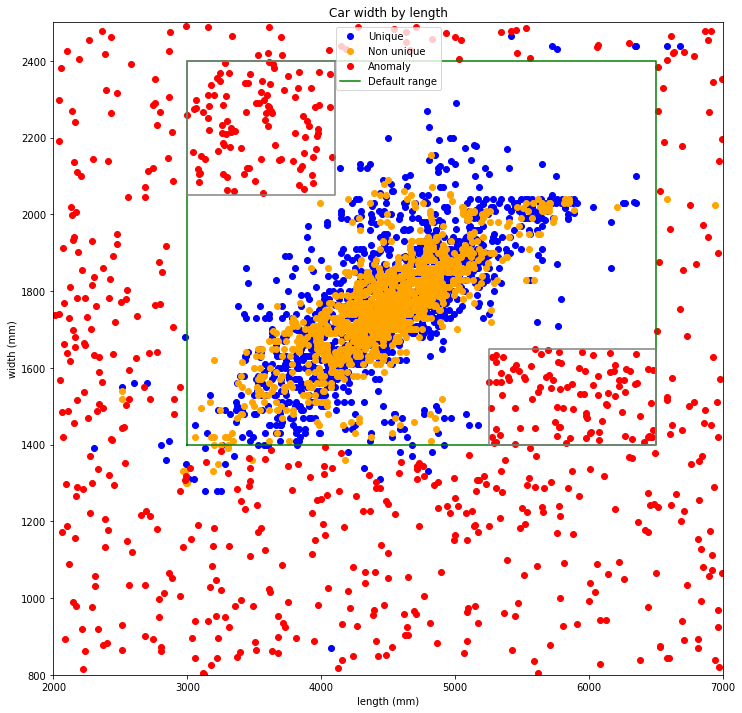
\includegraphics[width=\textwidth]{img/first_try.png}
\caption{Régions de décision manuelles pour des dimensions de voitures\label{regions_decision_manuelles_plot}}
\end{figure}

\section{Recherche des bases de données}

\section{Environnement de travail}

Dans cette partie, nous décrivons les outils utilisés et développés pour poursuivre notre étude. Ces éléments se retrouvent sur le dépôt git que nous avons utilisé pour sauvegarder notre code : \href{https://github.com/ychalier/anomaly/}{github.com/ychalier/anomaly}.

\subsection{Environnement Python}

Afin d'éviter d'éventuels problème de version, nous avons opté pour l'utilisation d'environnements virtuels à l'aide du module \texttt{virtualenv}. Nous avons choisi le noyau Python 3.6. Les modules utilisés sont regroupés dans le fichier requirements.txt présent dans le dépôt git. Les principaux sont :
\begin{itemize}
\item \texttt{numpy}
\item \texttt{pandas}
\item \texttt{matplotlib}
\item \texttt{jupyter}
\item \texttt{scikit-learn}
\end{itemize}

\subsection{Chargement des bases de données}

Afin de centraliser le chargement des bases de données explicitées plus tôt entre tous les scripts en ayant besoin, nous avons implémenté une fonction de chargement nommée \texttt{load\_detector} dans loader.py. Cette fonction instancie un object de la classe Detector, que nous décrirons dans la partie suivante. Elle procède de la façon suivante :

\begin{enumerate}
\item Pour chaque jeu de données au format CSV
\begin{enumerate}[{1.}1.]
\item Lire les colonnes contenant la longueur et la largeur
\item Renommer ces colonnes en "\texttt{length}" et "\texttt{width}"
\item Supprimer les lignes incomplètes
\item Si nécessaire, convertir les données en flottant et en millimètres
\item Ajouter une colonne contenant la classe correspondant au jeu de données considéré
\item Appliquer un premier filtre sur la longueur ou la largeur pour supprimer les points extrêmes isolés
\end{enumerate}
\item Fusionner toutes les matrices précédentes en une seule
\item Créer un nouvel objet \texttt{Detector} avec cette matrice en attribut
\item Supprimer les éventuels redondances
\item Ajouter une colonne "\texttt{odd}" à la matrice, initialisée à \texttt{False}
\item \textbf{Générer les données malicieuses}
\item Ajouter les données malicieuses à la base de données, en rajoutant la colonne "\texttt{odd}" initialisée à \texttt{True}
\item Remplacer les valeurs des classes (originnellement des chaînes de caractères comme \texttt{"car"} ou \texttt{"human"}) par des entiers
\item \textbf{Séparer la matrice en un jeu d'entraînement et un jeu de test}
\item Renvoyer l'objet `Detector` ainsi initialisé
\end{enumerate}

Dans le cas des bases de données décrites au paragraphe précédent, l'étape 1.6. permet de supprimer quelques points, par exemple une moto de longueur supérieure à 20 mètres, ou une voiture de 6 mètres de large. Bien que réelles, ces données sont trop isolées pour être considérés dans le reste de notre travail.

La DataFrame finale possède 4 colonnes, plus une pour l'index. Ces colonnes sont la classe du véhicule (entier), la longueur (flottant), la largeur (flottant), et le caractère malicieux (booléen).

\paragraph{Génération des données malicieuses} Pour un nombre de points à générer donné, le programme génère des points uniformément dans la zone rectangulaire définie par les minimums et maximums de longueur et de largeur de la base de données initiales. À chacun de ces points est associé, uniformément, une classe aléatoire parmi les classes présentes dans la base de données. La génération utilise un \emph{seed} entier entre 0 et $2^{32}-1$, ré-utilisable ultérieurement pour générer le même jeu de données.

\paragraph{Séparation de la matrice} Avec le \emph{seed} généré précédemment, la grande matrice est tout d'abord mélangée pour éviter d'avoir toutes les données triées. Puis, elle est coupée en deux moitiés :
\begin{itemize}
\item le jeu d'entraînement
\item le jeu de test
\end{itemize}
Enfin, on procède à la division de chacune de ces matrices en deux matrices, une pour les \emph{features} et une pour le label de sortie (le caractère malicieux). Au final, chacune de ces DataFrames (\texttt{x\_train}, \texttt{y\_train}, \texttt{x\_test} et \texttt{y\_test}) est stockée dans l'objet \texttt{Detector}.

\subsection{Classe \texttt{Detector}}

Comme expliqué précédemment, cette classe stocke les jeux de données utilisés pour l'entraînement et la prédiction. Elle va aussi permettre de centraliser les tests de \emph{classifiers}, et l'affichage des données. Ses méthodes (Table \ref{methodes_detector}) sont donc une sorte d'API pour la réalisation de la fonction de prédiction finale, objectif du projet.

\begin{table}[h]
\centering
\begin{tabular}{p{2.3cm} p{3.1cm} p{4.6cm}}

\multirow{6}{*}{Pre-processing}& \multirow{2}{*}{\texttt{clean}} & Étapes 4 et 5 du chargement des données \\
& \multirow{2}{*}{\texttt{append\_odd\_points}} & Étape 7 du chargement des données \\
& \multirow{2}{*}{\texttt{format}} & Étapes 8 et 9 du chargement des données \\
\hline
& \multirow{2}{*}{\texttt{classify}} & Entraîne un \emph{classifier} et renvoie le score de test\\
Interface \par \texttt{sklearn} & \multirow{2}{*}{\texttt{tune\_parameters}} & Trouve le meilleur jeu de paramètres pour un \emph{classifier}\\
& \multirow{2}{*}{\texttt{predict}} & Fonction finale de prédiction online \\
\hline
\multirow{4}{*}{Affichage}& \multirow{2}{*}{\texttt{plot}} & Affiche la matrice de données complètes\\
& \texttt{plot\_decision\_}\par\texttt{boudaries} & Affiche les régions de décisions d'un \emph{classifier}\\

\end{tabular}
\caption{Méthodes de la classe \texttt{Detector}\label{methodes_detector}}
\end{table}

\section{Méthode d'évaluation}

\chapter{Paramétrage et résultats}

\section{Recherche des paramètres optimaux}

Une majeure partie de notre temps a été investie dans la recherche des jeux de paramètres optimaux pour chacun des \emph{classifiers} sélectionnés. Nous avons procédé en deux temps. Premièrement, nous avons implémenté un script testant des intervalles de paramètres et renvoyant les meilleurs combinaisons. Puis, nous avons utilisé ce script pour des intervalles de valeurs de paramètres que nous avons jugé pertinents.

\subsection{Recherche exhaustive et validation croisée}

Notre algorithme de recherche des paramètres est basé sur une fonction de scikit-learn, dans le module de sélection de modèle : \texttt{GridSearchCV}. Cette fonction est utilisée dans la méthode \texttt{tune\_parameters} du \texttt{Detector}. Cette fonction effectue une recherche exhaustive d'un jeu de paramètres optimal pour un \emph{classifier} donné à partir d'un dictionnaire dont les clés sont les paramètres à faire varier et les valeurs les listes des valeurs prises par ces paramètres.

Cette fonction utilise de plus la technique de validation croisée. En quelques mots, cette technique consiste en la division des données d'entraînement en $C$ sous-échantillons. 1 sous-échantillon servira à la validation du modèle, tandis que les $C-1$ autres permettront l'entraînement du modèle. On répète cette opération $C$ fois, afin que chaque sous-échantillon soit utilisé pour la validation une fois. La performance du modèle est ensuite évaluée en effectuant la moyenne des $C$ erreurs quadratiques.

La fonction d'évaluation du score utilisée par \texttt{GridSearchCV} est par ailleurs modifiable. Dans le cadre de notre projet, nous nous intéressons au \emph{f1-score} pour évaluer un modèle, et nous souhaitions aussi extraire, si possible, les tendances d'évolution du score en fonction des différents paramètres testés. Nous avons donc implémenté notre propre fonction d'évaluation, prenant en paramètre l'estimateur à évaluer et les matrices de \emph{features} et de \emph{labels} à utiliser pour cela. Cette fonction effectue les opérations suivantes :

\begin{enumerate}
\item Prédiction des \emph{labels} à partir de la matrice de \emph{features}
\item Calcul de la matrice de confusion entre la prédiction et la matrice donnée en consigne
\item \textbf{Sauvegarde des paramètres et du score}
\item Retour du \emph{f1-score}
\end{enumerate}

L'étape 3 consiste en l'écriture dans un fichier d'une ligne contenant la description détaillée des paramètres de l'estimateur ainsi que les résultats des scores. La fonction de recherche exhaustive étant fortement parallèle, chaque processus écrit dans son propre fichier. Une fois tous les tests effectués, ces fichiers sont concaténés en un grand fichier. Cette méthode d'enregistrement continu permet en outre de sauvegarder les résultats des tests au fur et à mesure de l'exécution du programme, ce qui se révèlera important lors d'interruptions prématurées de cette exécution.

En effet, ce fut l'un de nos plus importants problèmes lors de ce projet. Pour le Multi-layered Perceptron, il y avait beaucoup de paramètres en jeu, et la complexité combinatoire mélangée avec le temps de convergence des réseaux neuronaux ont rendu l'exécution du script interminables. Notre plus long essai eut lieu sur le serveur InfRes \href{http://lame10.enst.fr}{lame10} doté pourtant de 80 cpus, sur une durée de plus de 18 heures. Malgré tout, il aura fallut interrompre l'exécution du programme manuellement pour rendre le serveur disponible. Le fichier généré pesait plus de 120Mo, et les deux CSV extraits pèsent respectivement 25Mo et 23Mo.

Enfin, du grand fichier généré contenant l'historique de tous les tests passés sont ensuite extraites les tables de score CSV qui seront présentées dans les paragraphes suivant. Ces dernières sont disponibles à l'adresse \url{https://perso.telecom-paristech.fr/ychalier/anomaly/params/}. Pour chaque phase de test, le script génère :
\begin{itemize}
\item Un fichier de scores (TPR, FPR, TNR, FNR, PPV, \emph{f1-score}, temps de prédiction)
\item Pour chaque classe différente d'estimateur, un fichier contenant tous les jeux de paramètres
\end{itemize}
Ces tables sont, à la manière des tables en SQL, liées par une clé primaire externe qui est l'identifiant (unique) de la combinaison de paramètres.

%TODO : perspective : bloquer les paramètres reconnus comme meilleurs et faire varier ceux qui semblent useless, peut-être qu'une tendance va émerger

\subsection{Multi-layered perceptron}

À l'aide d'un autre petit script Python, nous avons pu afficher les données récoltées dans les CSV mentionnés plus tôt. Les Figures \ref{mlp_activation} et \ref{mlp_solver} sont le résultat du long test pour les paramètres du MLP. La Table \ref{params_mlp} regroupe les différents paramètres testés.

\begin{table}[h]
\centering
\begin{tabular}{ll}
paramètre & ensemble des valeurs testées \\
\hline
\texttt{learning\_rate} & \texttt{'constant'}, \texttt{'invscaling'} et \texttt{'adaptive'}\\
\texttt{alpha} & $\{10^{-k} \>\> | \>\> k \in [\![4, 7]\!] \}$ \\
\texttt{activation} & \texttt{'identity'}, \texttt{'logistic'}, \texttt{'tanh'} et \texttt{'relu'} \\
\texttt{solver} & \texttt{'lbfgs'}, \texttt{'sgd'} et \texttt{'adam'}\\
\texttt{hidden\_layer\_sizes} & 0 à 5 \emph{layers}, de taille variant de 1 à 49\\
\end{tabular}
\caption{Liste des paramètres testés pour le multi-layered perceptron\label{params_mlp}}
\end{table}

\begin{figure}
\centering
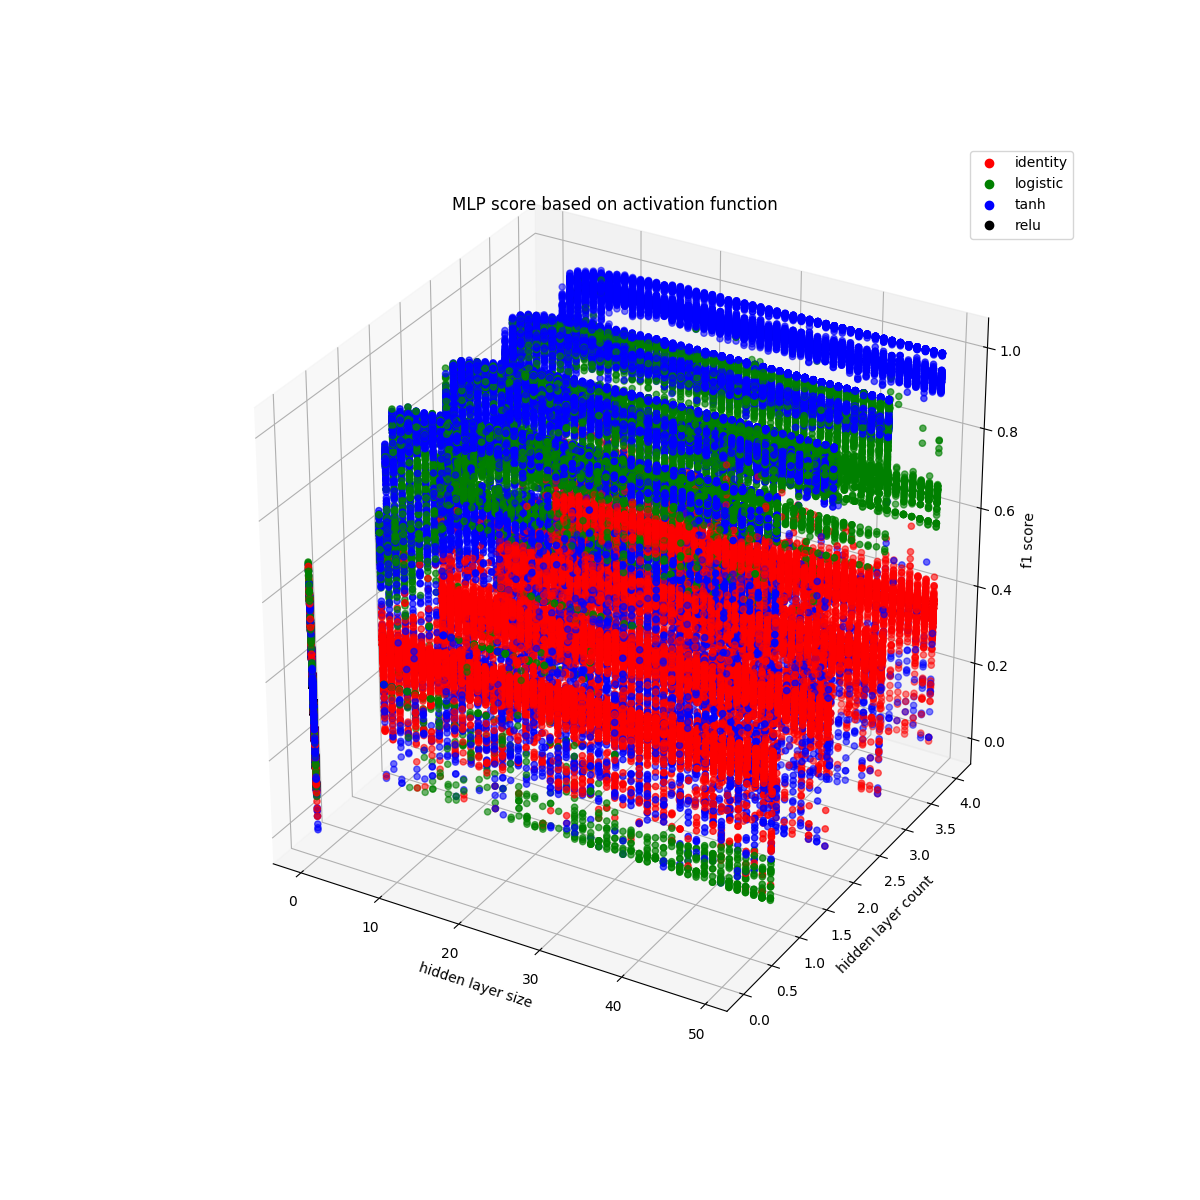
\includegraphics[width=\textwidth]{img/mlp_activation.png}
\caption{Évolution du score pour MLP selon la fonction d'activation\label{mlp_activation}}
\end{figure}

\begin{figure}
\centering
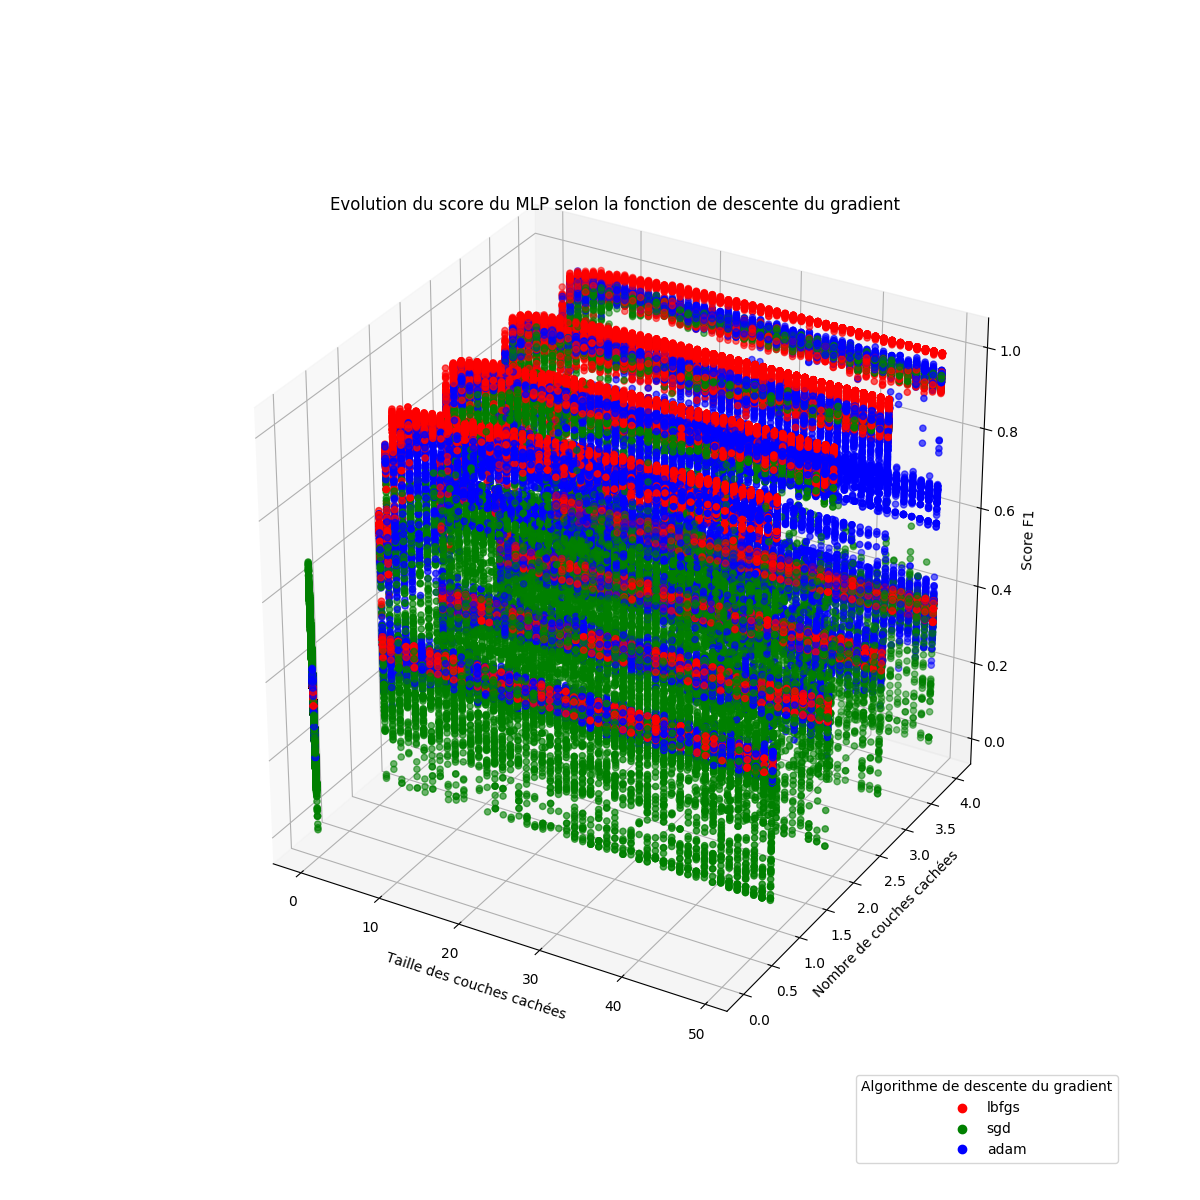
\includegraphics[width=\textwidth]{img/mlp_solver.png}
\caption{Évolution du score pour MLP selon l'algorithme de descente du gradient\label{mlp_solver}}
\end{figure}

L'exploitation des résultats est rendue très difficile par le manque de consistance des scores. Cependant, nous avons pu remarqués que des paramètres comme la régularisation (\texttt{alpha}) ou la taille et nombre de \emph{layers} n'avaient que peu d'influence sur les résultats. Par contre, deux éléments semblent ce dégager : \begin{itemize}
\item la tangente hyperbolique comme fonction d'activation
\item \emph{lbfgs} comme méthode du gradient (la documentation de sklearn prédit cette préférence lorsqu'il y a peu de données à exploiter)
\end{itemize}
Enfin, la Table \ref{best_params_mlp} donne les résultats donnés par la recherche exhaustive et validation croisée.

\begin{table}[h]
\centering
\begin{tabular}{ll}
paramètre & valeur \\
\hline
\texttt{learning\_rate} & \\
\texttt{alpha} &  \\
\texttt{activation} & \texttt{'tanh'} \\
\texttt{solver} & \texttt{'lbfgs'} \\
\texttt{hidden\_layer\_sizes} & \\
\end{tabular}
\caption{Paramètres optimaux pour MLP\label{best_params_mlp}}
\end{table}

%TODO : insister plus sur les problèmes de variance / inconsistence
%TODO : vérifier pour learning_rate / alpha

\subsection{AdaBoost}

Comme pour MLP, la Table \ref{params_ada} liste les paramètres testés et la Figure \ref{adaboost_depth} montre l'évolution du score en fonction de ces paramètres.

\begin{table}[h]
\centering
\begin{tabular}{ll}
paramètre & ensemble des valeurs testées \\
\hline
\texttt{n\_estimators} & $[\![1, 99]\!]$ \\
\texttt{learning\_rate} & $\{k/10 \>\> | \>\> k \in [\![1, 9]\!] \}$ \\
\texttt{base\_estimator} & Arbres de décision de profondeur maximale dans $[\![2, 9]\!]$\\
\end{tabular}
\caption{Liste des paramètres testés pour AdaBoost\label{params_ada}}
\end{table}

Ici, il y a peu d'interprétations possibles : les paramètres influent peu sur la performance de l'estimateur. Dès lors que les arbres sont suffisamment profonds, qu'il y a assez d'estimateurs agrégés et que le taux d'apprentissage et correct, les résultats sont vite optimaux. La fonction de recherche exhaustive nous a renvoyé la combinaison de paramètres présentée dans la Table \ref{best_params_ada} (pour un \emph{f1-score} moyen maximal de 0,947).

\begin{table}[h]
\centering
\begin{tabular}{ll}
paramètre & valeur \\
\hline
\texttt{n\_estimators} & 46 \\
\texttt{learning\_rate} & 0,3 \\
\texttt{base\_estimator} & Arbres de décision de profondeur maximale 3\\
\end{tabular}
\caption{Paramètres optimaux pour AdaBoost\label{best_params_ada}}
\end{table}

\begin{figure}
\centering
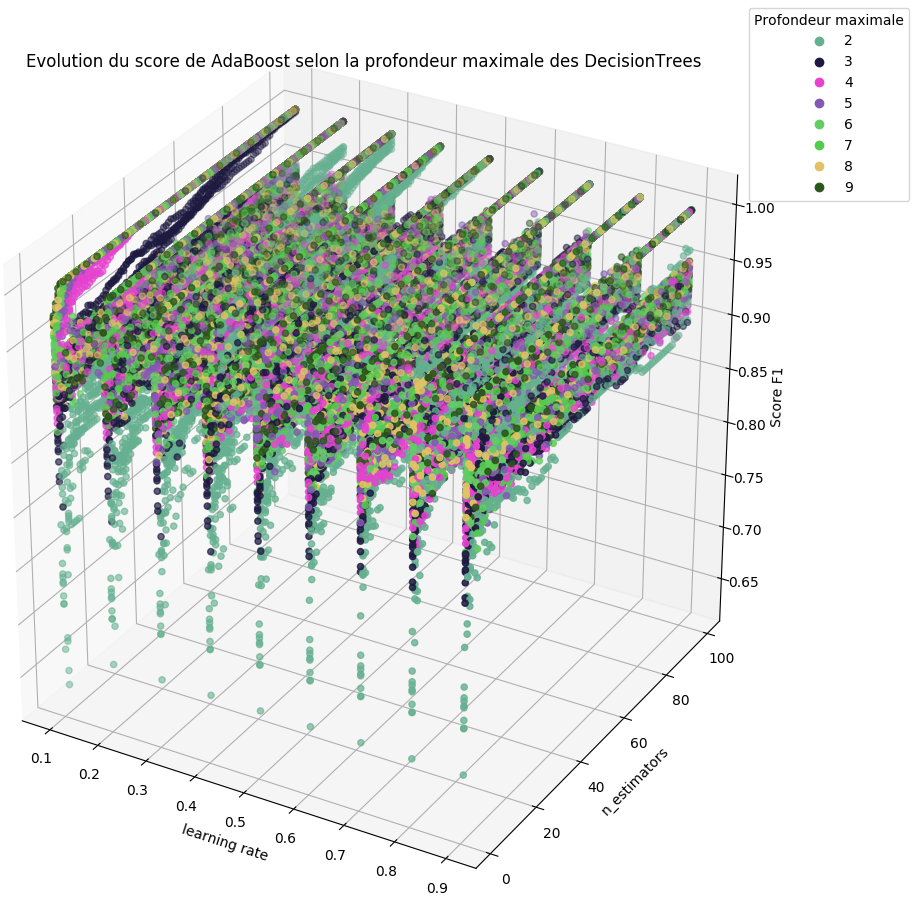
\includegraphics[width=\textwidth]{img/adaboost_depth.png}
\caption{Évolution du score pour AdaBoost selon la profondeur maximale de l'arbre de décision\label{adaboost_depth}}
\end{figure}

\subsection{SVM}

\section{Étude comparative des performances}

\section{Utilisation de la prédiction en-ligne}

L'objectif final de ce projet est la mise à disposition d'une fonction de prédiction autonome permettant de classer des données relevées par un ensemble de capteurs en malicieux / non-malicieux.

Cette fonction est déjà implémentée dans le code, il s'agit de la méthode \texttt{predict} de la classe \texttt{Detector}. Le processus pour initialiser cette fonction est le suivant :
\begin{enumerate}
\item Créer un objet \texttt{Detector} en chargeant les bases de données récoltées
\item Entraîner un \emph{classifier}, dont les paramètres sont ceux résultant de l'optimisation effectuée précédemment, avec ces données
\item Attribuer ce \emph{classifier} en tant que \emph{classifier} de prédiction pour le \texttt{Detector}
\item Sauvegarder la méthode \texttt{predict}
\end{enumerate}
La dernière étape de ce processus consiste en la sérialisation de la méthode, à l'aide du module \texttt{pickle}. La méthode, contenant une référence à l'estimateur sélectionné, possède tous les éléments pour effectuer les prédictions. Son utilisation peut alors être résumée à l'aide de la fonction suivante :
\begin{verbatim}
def classify(class_, length, width):
    import pickle
    file = open('anomaly_classifier.clf', 'rb')
    fun = pickle.load(file)
    file.close()
    if fun(class_, length, width):
        return "malicious"
    else:
        return "non-malicous"
\end{verbatim}
Cette fonction est autonome et portable; elle ne nécessite qu'un fichier contenant la méthode citée précédemment. 

% \begin{thebibliography}{9}
% \end{thebibliography}

\end{document}